\documentclass[margin=5pt]{standalone}
% \usepackage[a4paper]{geometry}
\usepackage[utf8]{inputenc}
\usepackage{xifthen}
\usepackage{tikz}
% \usetikzlibrary{patterns}
\usetikzlibrary{math,calc}

\title{Electoral College 2020 cartogram}
\author{Stuart Presnell}
\date{October 2020}


\newcommand{\U}[1]{++(0,#1)}
\newcommand{\D}[1]{++(0,-#1)}
\newcommand{\E}[1]{++(#1,0)}
\newcommand{\W}[1]{++(-#1,0)}

\begin{document}

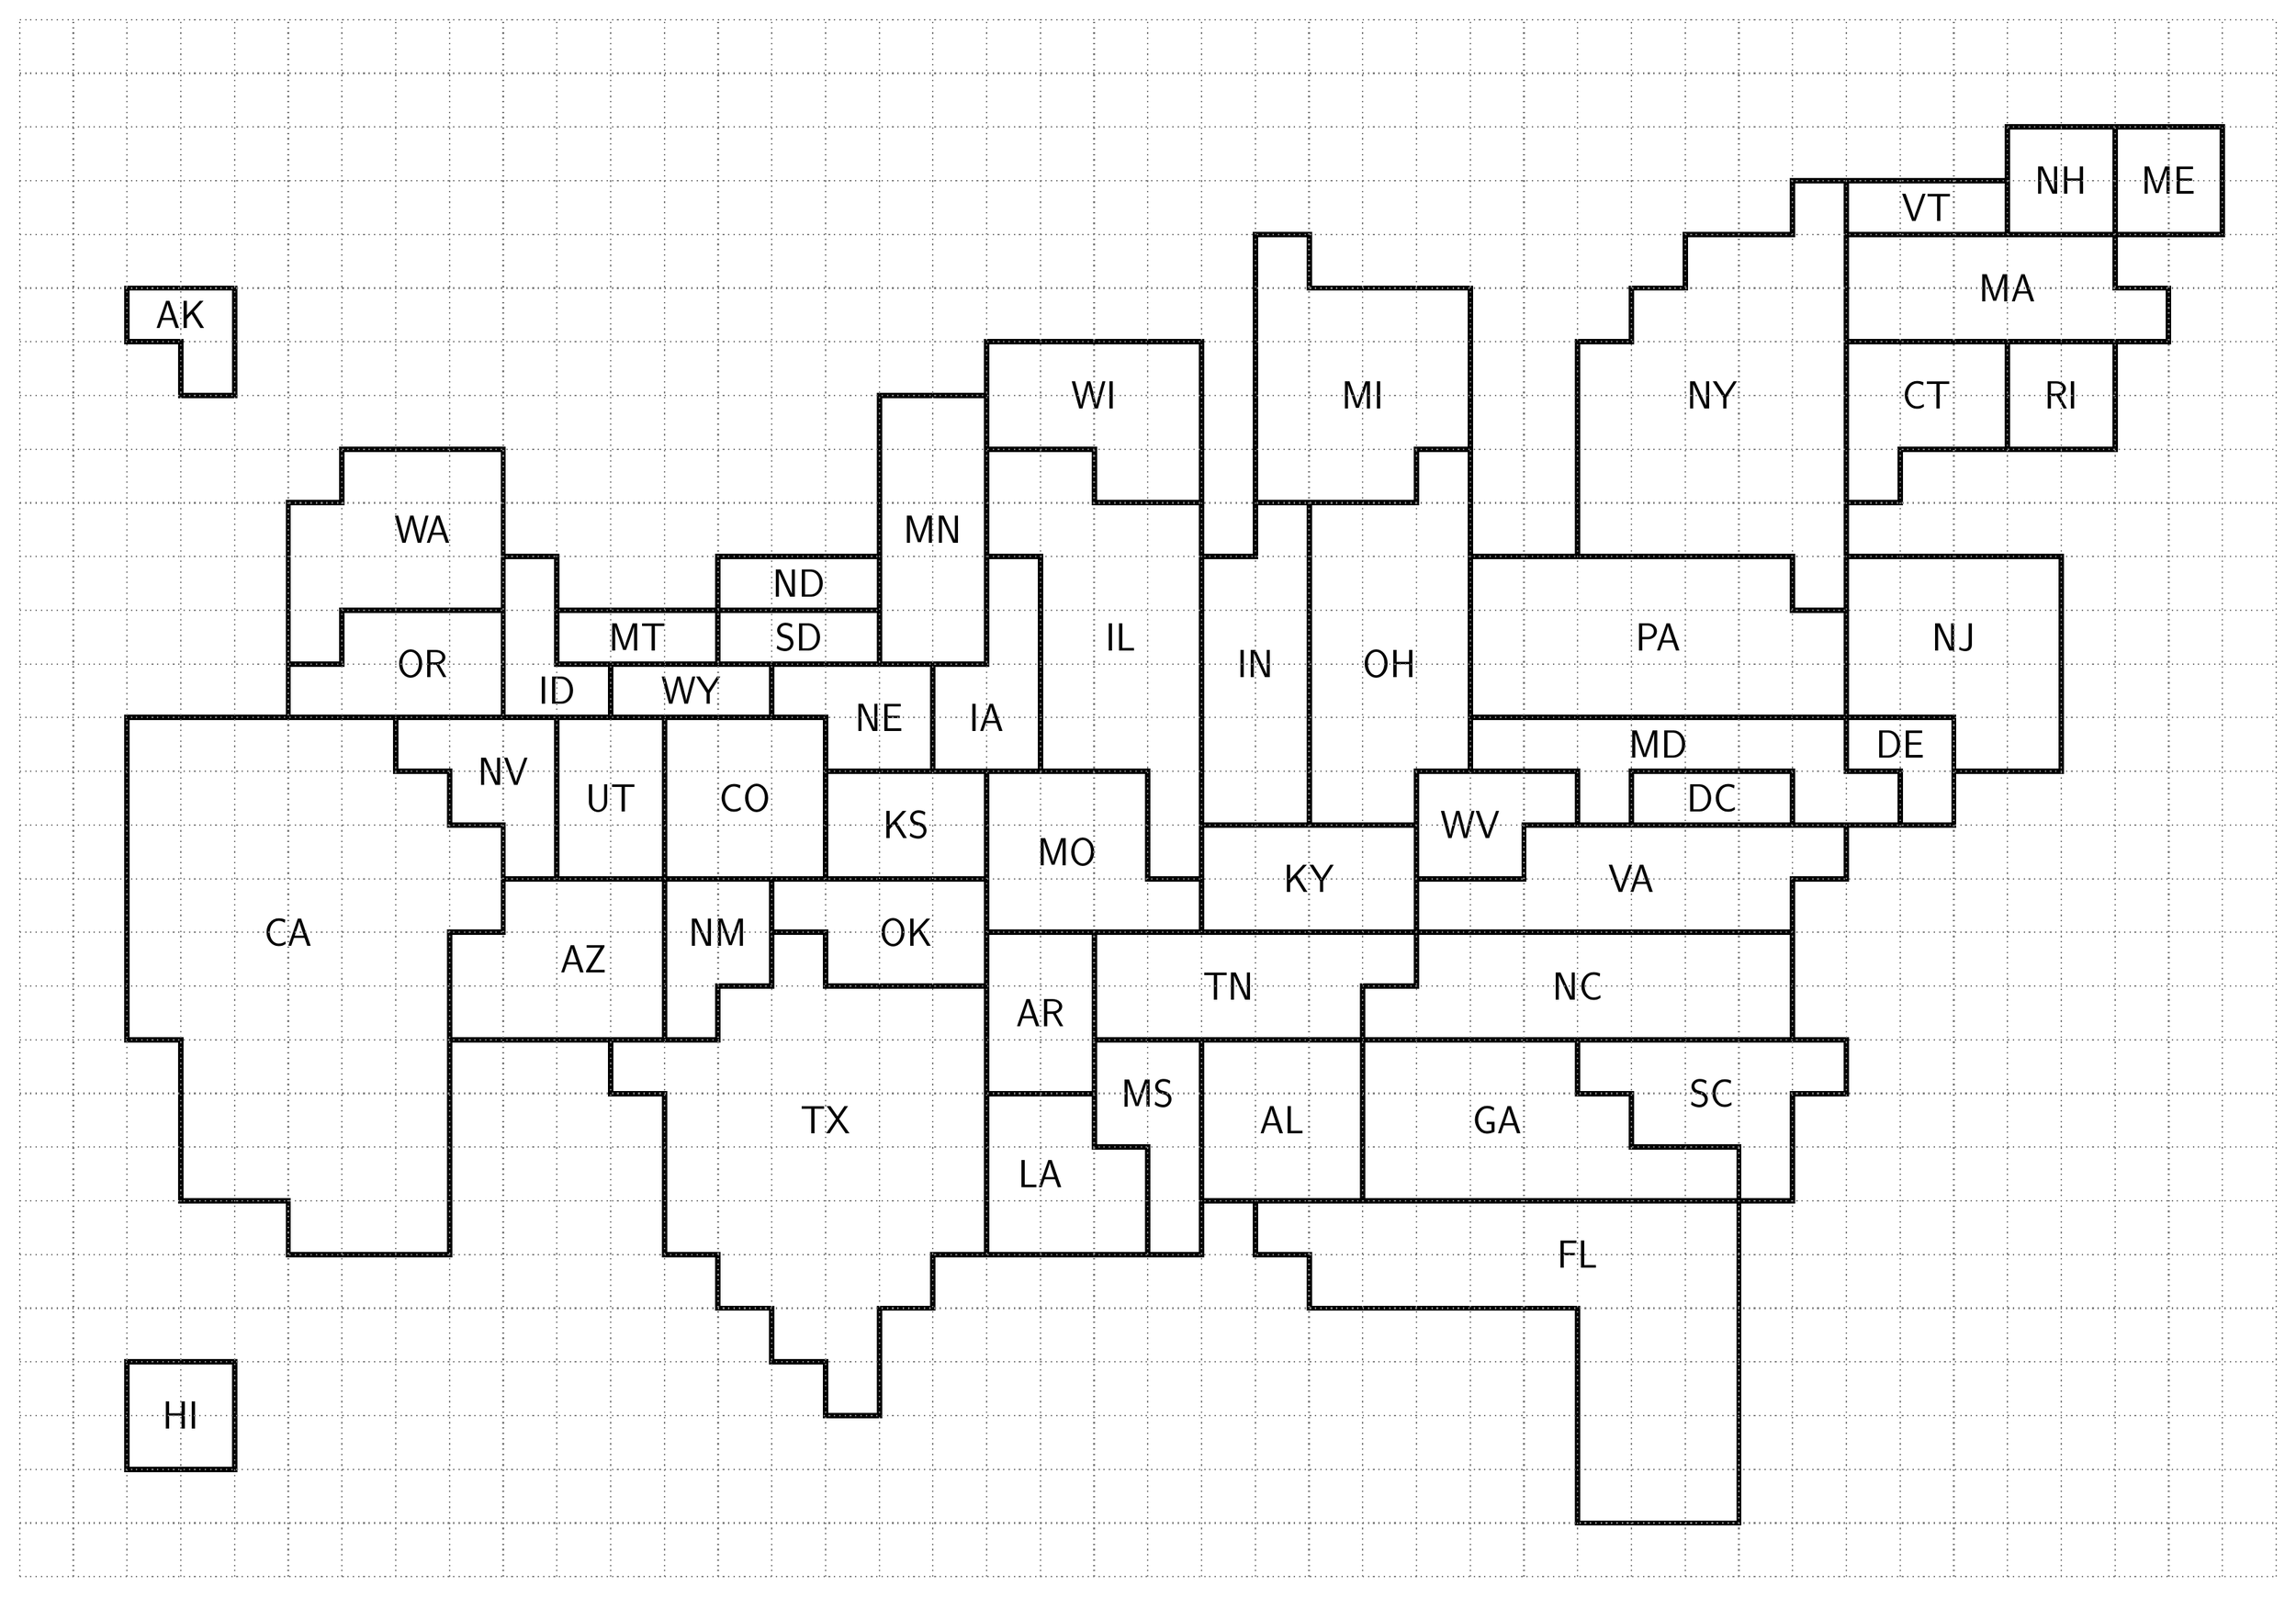
\begin{tikzpicture}\sffamily

\tikzstyle{wait}=[fill=white, font=\huge, text=black]
\tikzstyle{Dwin}=[fill=blue!70, font=\huge, text=yellow]
\tikzstyle{Rwin}=[fill=red!70, font=\huge, text=yellow]
\tikzstyle{Dfav}=[fill=cyan!10, font=\huge, text=black]
\tikzstyle{Rfav}=[fill=pink!40, font=\huge, text=black]



\tikzstyle{state}=[line width=1mm]
% \tikzstyle{lake}=[fill=white]
\tikzstyle{label}=[font=\huge, text=black]

% \tikzstyle{AK}=[wait]	% Alaska
\tikzstyle{AL}=[wait]	% Alabama
\tikzstyle{AR}=[Rfav]	% Arkansas
\tikzstyle{AZ}=[wait]	% Arizona
\tikzstyle{CA}=[Dfav]	% California
\tikzstyle{CO}=[Dfav]	% Colorado
\tikzstyle{CT}=[Dfav]	% Connecticut
\tikzstyle{DC}=[Dfav]	% District of Columbia*
\tikzstyle{DE}=[Dfav]	% Delaware
\tikzstyle{FL}=[wait]	% Florida
\tikzstyle{GA}=[wait]	% Georgia
\tikzstyle{HI}=[Dfav]	% Hawaii
\tikzstyle{IA}=[wait]	% Iowa
\tikzstyle{ID}=[Rfav]	% Idaho
\tikzstyle{IL}=[Dfav]	% Illinois
\tikzstyle{IN}=[wait]	% Indiana
\tikzstyle{KS}=[wait]	% Kansas
\tikzstyle{KY}=[wait]	% Kentucky
\tikzstyle{LA}=[wait]	% Louisiana
\tikzstyle{MA}=[Dfav]	% Massachusetts
\tikzstyle{MD}=[Dfav]	% Maryland
\tikzstyle{ME}=[Dfav]	% Maine**
\tikzstyle{MI}=[wait]	% Michigan
\tikzstyle{MN}=[wait]	% Minnesota
\tikzstyle{MO}=[wait]	% Missouri
\tikzstyle{MS}=[Rfav]	% Mississippi
\tikzstyle{MT}=[wait]	% Montana
\tikzstyle{NC}=[wait]	% North Carolina
\tikzstyle{ND}=[Rfav]	% North Dakota
\tikzstyle{NE}=[Rfav]	% Nebraska**
\tikzstyle{NH}=[wait]	% New Hampshire
\tikzstyle{NJ}=[Dfav]	% New Jersey
\tikzstyle{NM}=[Dfav]	% New Mexico
\tikzstyle{NV}=[wait]	% Nevada
\tikzstyle{NY}=[Dfav]	% New York
\tikzstyle{OH}=[wait]	% Ohio
\tikzstyle{OK}=[Rfav]	% Oklahoma
\tikzstyle{OR}=[Dfav]	% Oregon
\tikzstyle{PA}=[wait]	% Pennsylvania
\tikzstyle{RI}=[Dfav]	% Rhode Island
\tikzstyle{SC}=[wait]	% South Carolina
\tikzstyle{SD}=[Rfav]	% South Dakota
\tikzstyle{TN}=[Rfav]	% Tennessee
\tikzstyle{TX}=[wait]	% Texas
\tikzstyle{UT}=[Rfav]	% Utah
\tikzstyle{VA}=[Dfav]	% Virginia
\tikzstyle{VT}=[Dfav]	% Vermont
\tikzstyle{WA}=[Dfav]	% Washington
\tikzstyle{WI}=[wait]	% Wisconsin
\tikzstyle{WV}=[Rfav]	% West Virginia
\tikzstyle{WY}=[Rfav]	% Wyoming

\tikzstyle{AK}=[label]	% Alaska
\tikzstyle{AL}=[label]	% Alabama
\tikzstyle{AR}=[label]	% Arkansas
\tikzstyle{AZ}=[label]	% Arizona
\tikzstyle{CA}=[label]	% California
\tikzstyle{CO}=[label]	% Colorado
\tikzstyle{CT}=[label]	% Connecticut
\tikzstyle{DC}=[label]	% District of Columbia*
\tikzstyle{DE}=[label]	% Delaware
\tikzstyle{FL}=[label]	% Florida
\tikzstyle{GA}=[label]	% Georgia
\tikzstyle{HI}=[label]	% Hawaii
\tikzstyle{IA}=[label]	% Iowa
\tikzstyle{ID}=[label]	% Idaho
\tikzstyle{IL}=[label]	% Illinois
\tikzstyle{IN}=[label]	% Indiana
\tikzstyle{KS}=[label]	% Kansas
\tikzstyle{KY}=[label]	% Kentucky
\tikzstyle{LA}=[label]	% Louisiana
\tikzstyle{MA}=[label]	% Massachusetts
\tikzstyle{MD}=[label]	% Maryland
\tikzstyle{ME}=[label]	% Maine**
\tikzstyle{MI}=[label]	% Michigan
\tikzstyle{MN}=[label]	% Minnesota
\tikzstyle{MO}=[label]	% Missouri
\tikzstyle{MS}=[label]	% Mississippi
\tikzstyle{MT}=[label]	% Montana
\tikzstyle{NC}=[label]	% North Carolina
\tikzstyle{ND}=[label]	% North Dakota
\tikzstyle{NE}=[label]	% Nebraska**
\tikzstyle{NH}=[label]	% New Hampshire
\tikzstyle{NJ}=[label]	% New Jersey
\tikzstyle{NM}=[label]	% New Mexico
\tikzstyle{NV}=[label]	% Nevada
\tikzstyle{NY}=[label]	% New York
\tikzstyle{OH}=[label]	% Ohio
\tikzstyle{OK}=[label]	% Oklahoma
\tikzstyle{OR}=[label]	% Oregon
\tikzstyle{PA}=[label]	% Pennsylvania
\tikzstyle{RI}=[label]	% Rhode Island
\tikzstyle{SC}=[label]	% South Carolina
\tikzstyle{SD}=[label]	% South Dakota
\tikzstyle{TN}=[label]	% Tennessee
\tikzstyle{TX}=[label]	% Texas
\tikzstyle{UT}=[label]	% Utah
\tikzstyle{VA}=[label]	% Virginia
\tikzstyle{VT}=[label]	% Vermont
\tikzstyle{WA}=[label]	% Washington
\tikzstyle{WI}=[label]	% Wisconsin
\tikzstyle{WV}=[label]	% West Virginia
\tikzstyle{WY}=[label]	% Wyoming





\def\xmin{0};
\def\xmax{42};
\def\ymin{-1};
\def\ymax{28};

% \draw[step=1cm,gray,dotted,thick] (\xmin,\ymin) grid (\xmax,\ymax);
% \draw[step=2mm,gray,very thin] (\xmin,\ymin) grid (\xmax,\ymax);
% \draw[thick] (\xmin,0) -- (\xmax,0);
% \draw[thick] (0,\ymin) -- (0,\ymax);

% HI
\draw[state, HI] (2,1) rectangle ++(2,2);
\node[HI] at (3,2) (HI) {HI};

% AK
\draw[state, AK] (2,23) -- \D{1} -- \E{1} -- \D{1} -- \E{1} -- \U{2} -- cycle;
\node[AK] at (3,22.5) (AK) {AK};

% CA
\draw[state, CA] (2,15) -- \D{6} -- \E{1} -- \D{3} -- \E{2} -- \D{1} -- \E{3} -- \U{6} -- \E{1} -- \U{2} 
-- \W{1} -- \U{1} -- \W{1} -- \U{1} -- cycle;
\node[CA] at (5,11) (CA) {CA};


% OR
\draw[state, OR] (5,15) -- \E{4} -- \U{2} -- 
\W{3} -- \D{1} -- \W{1} -- cycle;
\node[OR] at (7.5,16) (OR) {OR};


% WA
\draw[state, WA] (5,16) -- \E{1} -- \U{1} -- \E{3} -- \U{3} -- 
\W{3} -- \D{1} -- \W{1} -- cycle;
\node[WA] at (7.5,18.5) (WA) {WA};


% AZ
\draw[state, AZ] (8,9) -- \E{4} -- \U{3} -- \W{3} --
\D{1} -- \W{1} -- cycle;
\node[AZ] at (10.5,10.5) (AZ) {AZ};


% NV
\draw[state, NV] (7,15) -- 
\D{1} -- \E{1} -- 
\D{1} -- \E{1} -- 
\D{1} -- \E{1} -- \U{3} -- cycle;
\node[NV] at (9,14) (NV) {NV};

% ID
\draw[state, ID] (9,15) -- \E{2} -- 
\U{1} -- \W{1} --
\U{2} -- \W{1} -- cycle;
\node[ID] at (10,15.5) (ID) {ID};


% UT
\draw[state, UT] (10,12) rectangle ++(2,3);
\node[UT] at (11,13.5) (UT) {UT};

% CO
\draw[state, CO] (12,12) rectangle ++(3,3);
\node[CO] at (13.5,13.5) (CO) {CO};

% NM
\draw[state, NM] (12,12) --
\D{3} -- \E{1} -- 
\U{1} -- \E{1} -- 
\U{2} -- \W{2} -- cycle;
\node[NM] at (13,11) (NM) {NM};

% MT
\draw[state, MT] (10,16) rectangle ++(3,1);
\node[MT] at (11.5,16.5) (MT) {MT};

% WY
\draw[state, WY] (11,15) rectangle ++(3,1);
\node[WY] at (12.5,15.5) (WY) {WY};

% SD
\draw[state, SD] (13,16) rectangle ++(3,1);
\node[SD] at (14.5,16.5) (SD) {SD};

% ND
\draw[state, ND] (13,17) rectangle ++(3,1);
\node[ND] at (14.5,17.5) (ND) {ND};

% NE
\draw[state, NE] (14,15) -- 
\E{1} -- \D{1} --
\E{2} -- \U{2} -- \W{3} -- cycle;
\node[NE] at (16,15) (NE) {NE};

% KS
\draw[state, KS] (15,12) rectangle ++(3,2);
\node[KS] at (16.5,13) (KS) {KS};

% OK
\draw[state, OK] (14,11) -- 
\E{1} -- \D{1} --
\E{3} -- \U{2} -- \W{4} -- cycle;
\node[OK] at (16.5,11) (OK) {OK};

% TX
\draw[state, TX] (11,9) -- 
\D{1} -- \E{1} -- 
\D{3} -- \E{1} -- 
\D{1} -- \E{1} -- 
\D{1} -- \E{1} -- 
\D{1} -- \E{1} -- 
\U{2} -- \E{1} -- 
\U{1} -- \E{1} -- 
\U{5} -- \W{3} -- 
\U{1} -- \W{1} -- 
\D{1} -- \W{1} -- 
\D{1} -- 
cycle;
\node[TX] at (15,7.5) (TX) {TX};


% MN
\draw[state, MN] (16,16) rectangle ++(2,5);
\node[MN] at (17,18.5) (MN) {MN};

% IA
\draw[state, IA] (17,14) -- 
\E{2} -- 
\U{4} -- \W{1} -- 
\D{2} -- \W{1} -- 
cycle;
\node[IA] at (18,15) (IA) {IA};

% MO
\draw[state, MO] (18,11)-- 
\E{4} -- 
\U{1} -- \W{1} --
\U{2} -- \W{3} -- cycle;
\node[MO] at (19.5,12.5) (MO) {MO};

% AR
\draw[state, AR] (18,8) rectangle ++(2,3);
\node[AR] at (19,9.5) (AR) {AR};

% LA
\draw[state, LA] (18,5)-- 
\E{3} -- 
\U{2} -- \W{1} --
\U{1} -- \W{2} -- cycle;
\node[LA] at (19,6.5) (LA) {LA};


% WI
\draw[state, WI] (18,20) -- 
\E{2} -- \D{1} --
\E{2} -- \U{3} -- \W{4} -- cycle;
\node[WI] at (20,21) (WI) {WI};


% IL
\draw[state, IL] (18,20) -- 
\D{2} -- \E{1} -- 
\D{4} -- \E{2} -- 
\D{2} -- \E{1} -- 
\U{7} -- \W{2} -- 
\U{1} -- 
cycle;
\node[IL] at (20.5,16.5) (IL) {IL};

% MI
\draw[state, MI] (23,19) -- 
\E{3} -- \U{1} -- \E{1} -- \U{3} -- 
\W{3} -- \U{1} -- \W{1} -- cycle;
\node[MI] at (25,21) (MI) {MI};

% IN
\draw[state, IN] (22,13) -- 
\E{2} -- \U{6} -- 
\W{1} -- \D{1} -- \W{1} -- cycle;
\node[IN] at (23,16) (IN) {IN};

% OH
\draw[state, OH] (24,13) -- 
\E{2} -- \U{1} -- \E{1} -- \U{6} -- 
\W{1} -- \D{1} -- \W{2} -- cycle;
\node[OH] at (25.5,16) (OH) {OH};

% KY
\draw[state, KY] (22,11) rectangle ++(4,2);
\node[KY] at (24,12) (KY) {KY};

% TN
\draw[state, TN] (20,11) --
\D{2} -- \E{5} -- 
\U{1} -- \E{1} -- 
\U{1} -- \W{6} -- 
cycle;
\node[TN] at (22.5,10) (TN) {TN};

% MS
\draw[state, MS] (20,7) -- 
\E{1} -- \D{2} --
\E{1} -- \U{4} -- \W{2} -- cycle;
\node[MS] at (21,8) (MS) {MS};

% AL
\draw[state, AL] (22,6) rectangle ++(3,3);
\node[AL] at (23.5,7.5) (AL) {AL};

% GA
\draw[state, GA] (25,6) -- 
\E{7} -- 
\U{1} -- \W{2} --
\U{1} -- \W{1} --
\U{1} -- \W{4} -- cycle;
\node[GA] at (27.5,7.5) (GA) {GA};

% SC
\draw[state, SC] (29,9) -- 
\D{1} -- \E{1} -- 
\D{1} -- \E{2} -- 
\D{1} -- \E{1} -- 
\U{2} -- 
\E{1} -- \U{1} -- 
cycle;
\node[SC] at (31.5,8) (SC) {SC};

% FL
\draw[state, FL] (23,6) -- 
\D{1} -- \E{1} -- \D{1} --
\E{5} -- \D{4} -- \E{3} -- \U{6} -- cycle;
\node[FL] at (29,5) (FL) {FL};


% NC
\draw[state, NC] (25,9) -- 
\E{8} -- \U{2} -- 
\W{7} -- \D{1} -- \W{1} -- cycle;
\node[NC] at (29,10) (NC) {NC};

% VA
\draw[state, VA] (26,11) -- 
\E{7} -- \U{1} -- 
\E{1} -- \U{1} -- 
\W{6} -- \D{1} -- \W{2} --
cycle;
\node[VA] at (30,12) (VA) {VA};


% WV
\draw[state, WV] (26,14) --
\D{2} -- \E{2} -- 
\U{1} -- \E{1} -- \U{1} -- \W{3} -- 
cycle;
\node[WV] at (27,13) (WV) {WV};

% DC
\draw[state, DC] (30,13) rectangle ++(3,1);
\node[DC] at (31.5,13.5) (DC) {DC};

% MD
\draw[state, MD] (27,15) -- 
\D{1} -- \E{2} -- 
\D{1} -- \E{1} -- 
\U{1} -- \E{3} -- 
\D{1} -- \E{2} -- 
\U{1} -- \W{1} -- 
\U{1} -- \W{7} -- 
cycle;
\node[MD] at (30.5,14.5) (MD) {MD};

% DE
\draw[state, DE] (34,14) -- 
\E{1} -- \D{1} --
\E{1} -- \U{2} -- \W{2} -- cycle;
\node[DE] at (35,14.5) (DE) {DE};

% PA
\draw[state, PA] (27,15)-- 
\E{7} -- 
\U{2} -- \W{1} --
\U{1} -- \W{6} -- cycle;
\node[PA] at (30.5,16.5) (PA) {PA};

% NJ
\draw[state, NJ] (34,15) -- 
\E{2} -- \D{1} --
\E{2} -- \U{4} -- \W{4} -- cycle;
\node[NJ] at (36,16.5) (NJ) {NJ};


% NY
\draw[state, NY] (29,18) -- 
\E{4} -- \D{1} --
\E{1} -- \U{8} -- \W{1} -- 
\D{1} -- \W{2} -- 
\D{1} -- \W{1} -- 
\D{1} -- \W{1} -- 
cycle;
\node[NY] at (31.5,21) (NY) {NY};

% VT
\draw[state, VT] (34,24) rectangle ++(3,1);
\node[VT] at (35.5,24.5) (VT) {VT};

% NH
\draw[state, NH] (37,24) rectangle ++(2,2);
\node[NH] at (38,25) (NH) {NH};

% ME
\draw[state, ME] (39,24) rectangle ++(2,2);
\node[ME] at (40,25) (ME) {ME};

% MA
\draw[state, MA] (34,22)-- 
\E{6} -- 
\U{1} -- \W{1} --
\U{1} -- \W{5} -- cycle;
\node[MA] at (37,23) (MA) {MA};

% CT
\draw[state, CT] (34,22) --
\D{3} -- \E{1} -- 
\U{1} -- \E{2} -- \U{2} -- \W{3} -- 
cycle;
\node[CT] at (35.5,21) (CT) {CT};

% RI
\draw[state, RI] (37,20) rectangle ++(2,2);
\node[RI] at (38,21) (RI) {RI};





% Grid:
\draw[step=1cm,gray,dotted,thick] (\xmin,\ymin) grid (\xmax,\ymax);

% % Lake Michigan
% \draw[state, lake] (22,18) rectangle ++(1,4);

% % Lake Erie / Lake Ontario
% \draw[state, lake] (27,18) rectangle ++(2,4);



\end{tikzpicture}

\end{document}










